\chapter{All-sky Analysis}
  \label{sec:analysis}
    What we present here is a test of the generalizability of results from Ch.\ref{ch:lori}, which focused on a particular structure on the sky, $\lambda$~Orionis.
    We first would like to note that ``all-sky analysis'' can be a bit misleading. The term tends to lead readers to the idea of a definitive study, answering a particular question for any given position on the sky.  While a truly all-sky analysis would be ideal, signal-to-noise constraints (mainly at high galactic latitudes), as well as confusion along the line of sight (mainly in the galactic plane), make a uniformly powerful study of the whole sky very challenging. Here we will indeed show results for the entire sky as a benchmark analysis, but for the core analysis we must mask certain regions dominated by systematic effects in order minimize biases for particular wavelenghts.

\section{Pixel masking and resolution}
    \subsubsection{Smoothing}
        As in Ch.~\ref{ch:lori}, this approach applies to a spatial resolution of approximately ~1$^{\circ}$. The resolution limimtation is imposed by the PC microwave component maps, which list an `effective resolution' of 60$'$ \citep{planck15X}. Thus we must apply a smoothing to most of our input datasets, which have native resolutions of a much finer scale (see Tab.~\ref{tab:data}), and Fig.~\ref{fig:AME_contours}. The data also come in a wide range of beam shapes with their own degrees of uncertainty, thus we conservatively smooth all of the data in the same way, using a circular Gaussian beam, to have ~1$^{\circ}$ FWHM resolution. we ar We start with an all-sky AME to IR comparison, looking for global patterns among all pixels.

    \subsection{Pixel mask}
        We prepare a global pixel mask (pixel positions masked in any map are excluded from the analysis).

      \paragraph{Zodical light}
        To keep our analysis comparable to previous works, we exclude pixels within 10$^{\circ}$ of the ecliptic plane \citep{hensley16}.  Even though we use the Zodi-subtracted maps \citep{kelsall98, kondo16, ootsubo16}, the Zodi residuals are still problematic (especially in the MIR.) This corresponds to regions with the heaviest contamination from Zodiacal light. Even in the Zodi-subtracted maps, residuals from the Zodi are apparent even with visual inspection for all of the MIR bands used in this study (see Ch.~\ref{ch:datasources} Ratio maps of MIR bands, in Figs. \ref{fig:ratioMap_A9I12}, and \ref{fig:ratioMap_A9I12}) demosntrate visually that the Zodi-residual patterns are quite different between AKARI and IRAS maps.

      \paragraph{Signal to noise}
        Some of the bands used lack sufficient sensitivity to trace fainter emisison, especially at higher galactic latitudes. This is mainly an issue for the mid-infrared bands. As such, we enforce a $3~\sigma$ threshold for all of the maps--- adding to the mask any pixel that has lower than $~\sigma$ detection in any of the maps.

     \paragraph{Point Sources}
       The Planck Collaboration provides masks of the pixels they find to include point sources. We mask pixels which are flagged as being point-source contaminated, in the most heavily affected maps: Planck/HFI 857 GHz and Planck/LFI 30 GHz.

  \section{All-sky cross correlations}

        In order to look more closely how the the AME to IR relationship varies with wavelength, we first do a comparison without applying any pixel mask, as a benchmark comparison. Fig.~\ref{fig:AMEvsDust_allsky_allbands_mpsub_kde_unmasked} shows the pizel-density plots of AME vs. the IR bands' intensities. Darker regions show higher pixel densities, unshaded or more lightly shaded regions show low or zero pixel densities. We see immediately that each band shows evidence of a positive trend with AME intensity, as in Ch.~\ref{ch:lori}. For the MIR bands, at lower IR intensities we see the effects of detector noise become dominant, turning into a more defined positive trend with increasing IR intensity. This effect is less pronounced in the FIR.
          \begin{figure}
            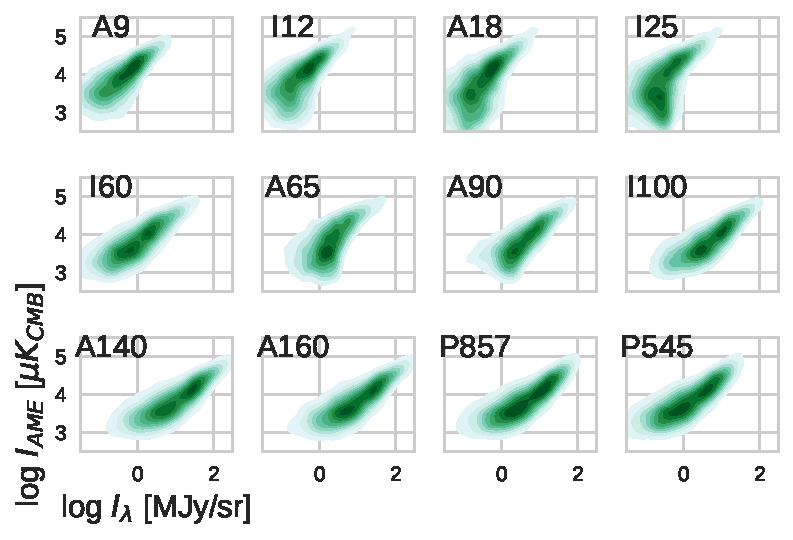
\includegraphics[width=\textwidth]{../Plots/ch_allsky/AMEvsDust_allsky_allbands_mpsub_kde_unmasked.pdf}
            \centering
            \caption{Point-density distributions of the AME intensity (Y-axis) vs. the IR bands' intensities. Darker regions indicated higher pixel densities. Only a simple mask of pixels near the ecliptic plane has been applied.}
            \label{fig:AMEvsDust_allsky_allbands_mpsub_kde_unmasked}
          \end{figure}
        We consider that the IR maps used must not only be compared to the AME, but to each other, to assess multi-wavelength patterns. We also compare the AME and IR maps to ancilliary maps, as decribed in Ch.~\ref{ch:datasources} and Tab.~\ref{tab:ancilliarydata}. Fig.~\ref{fig:all_bands_corr_matrix_wAME_spearman} confirms the weaker trend in the MIR vs. AME, via a cross-correlation matrix, similar to that used in Ch.~\ref{ch:lori} and Fig.~\ref{fig:orionis-corr-matrix}.
         Figure~\ref{fig:all_bands_corr_matrix_wAME_spearman} show the Spearman's $\rho$ ($r_{S}$) corrlation matrix for the unmasked sky.
          \begin{figure}
            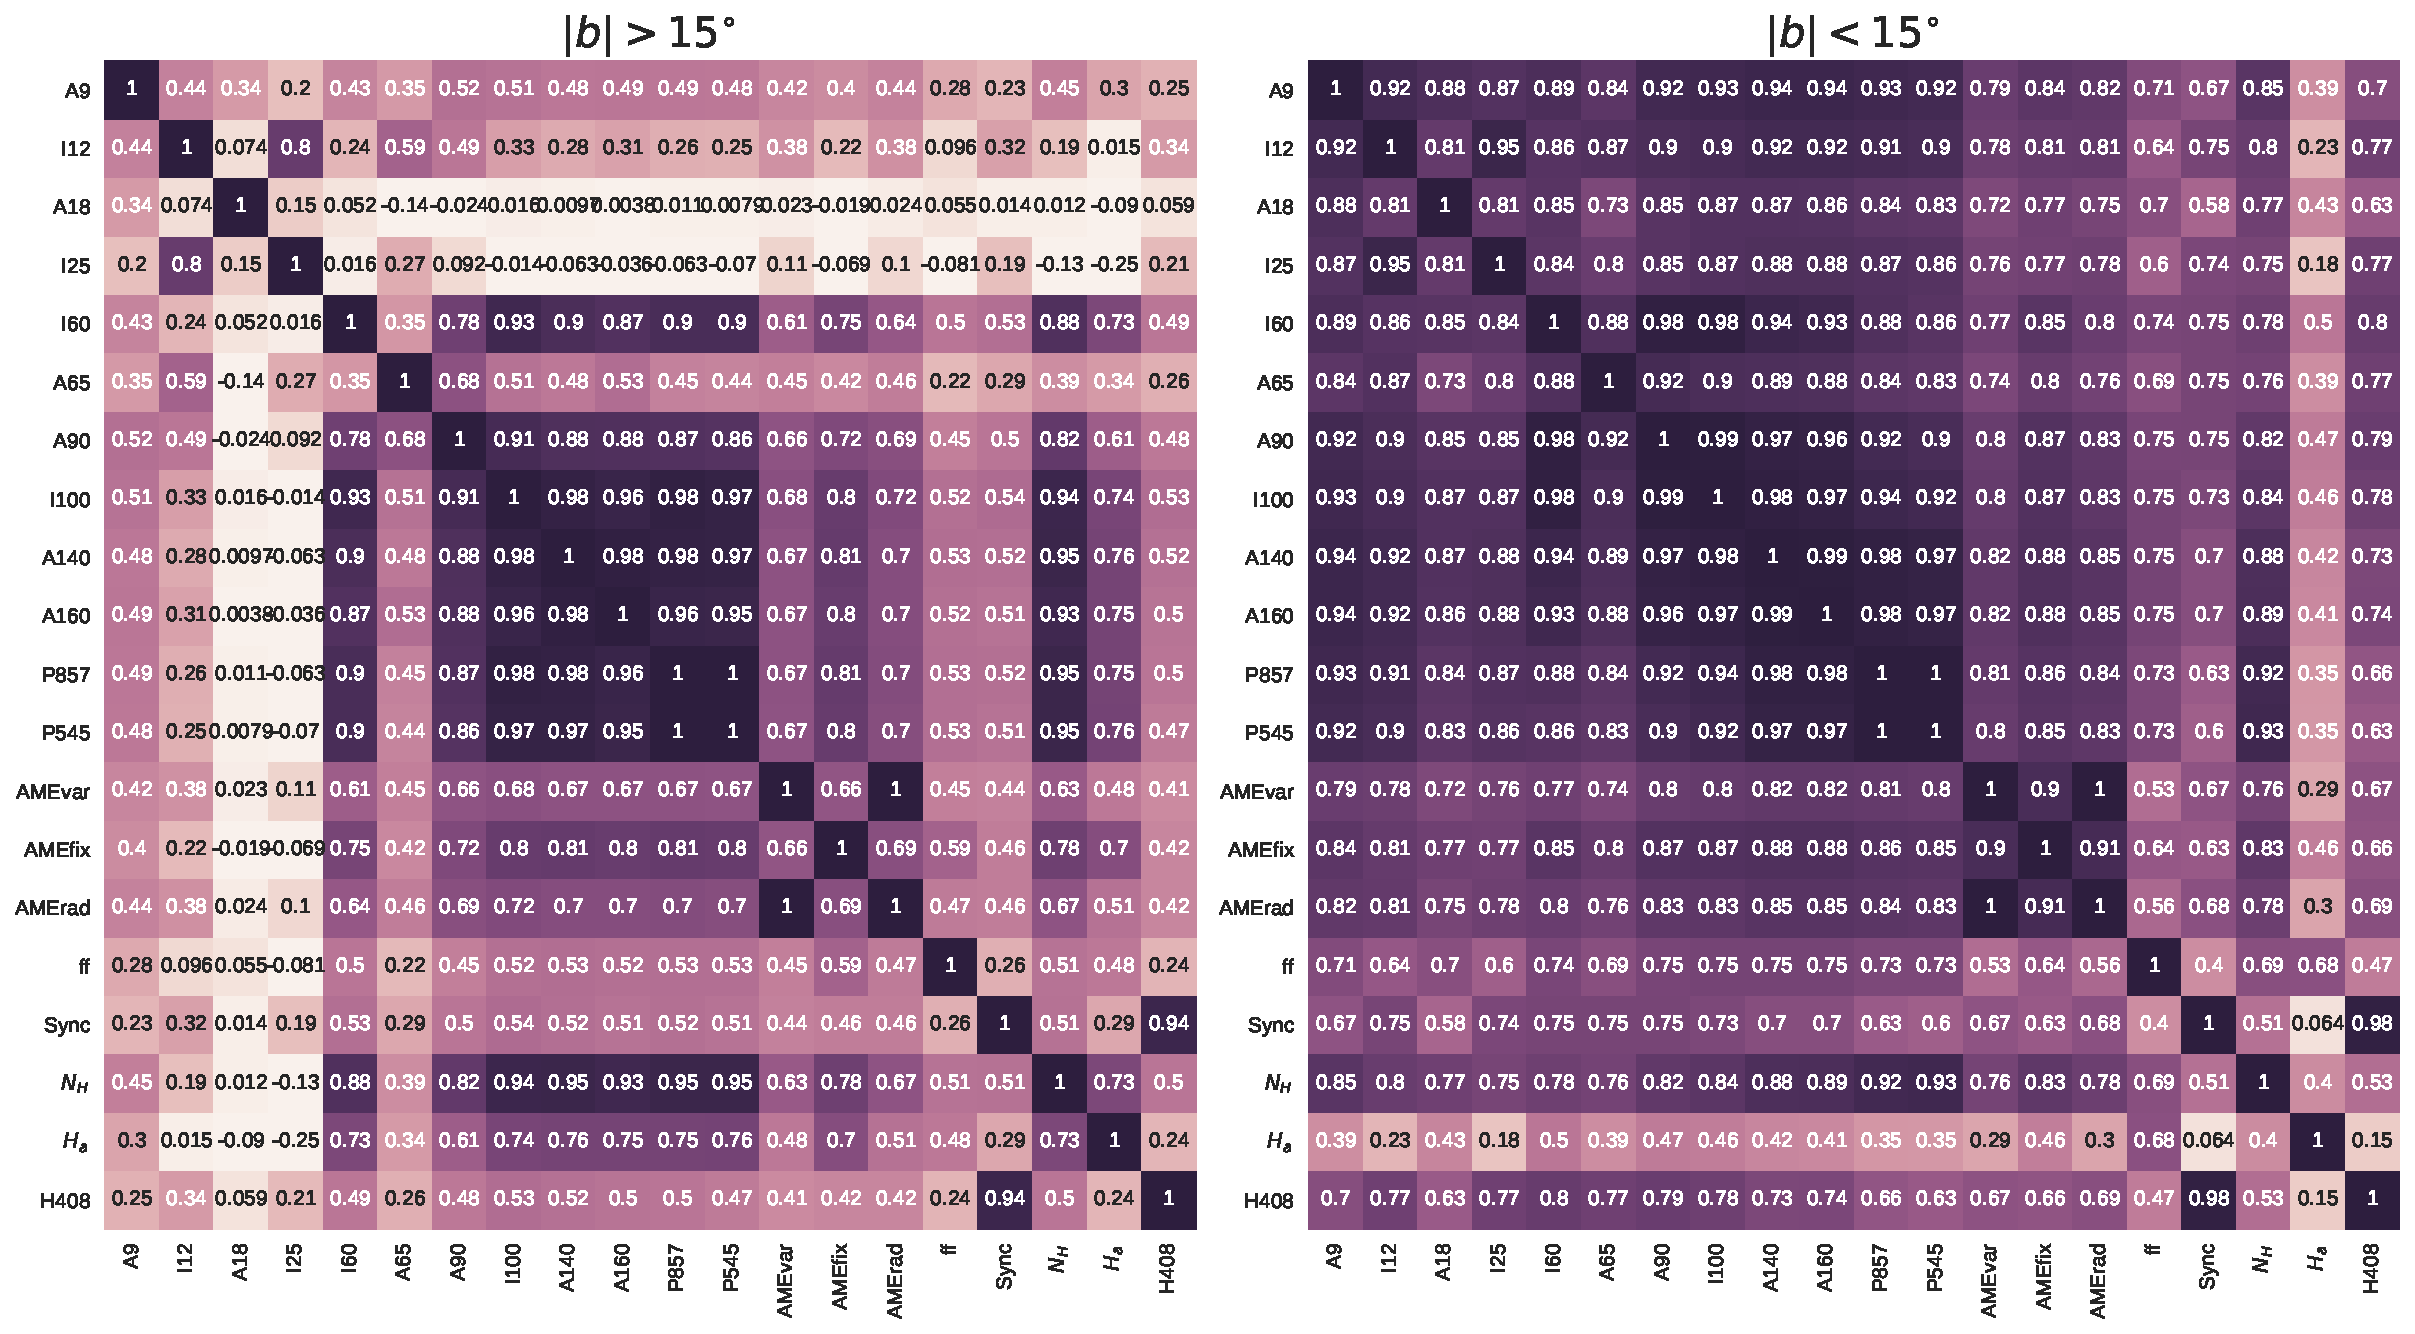
\includegraphics[width=\textwidth]{../Plots/ch_allsky/all_bands_corr_matrix_wAME_spearmanintensity_unmasked.pdf}
            \centering
            \caption{ALL-SKY cross-correlation matrix for the 12 infrared bands sampled, as well as the PC component maps (AME, Syncrotron, free-free), and ancilliary maps of $N_{H}$, $H_{\alpha}$ emission, and 408~MHz emission circa \cite{haslam82}. THe color-scale indicates ($r_{S}$). Results are based on the full sky (excluding pixels within 10$^{\circ}$ of the ecliptic plane). All-maps have been reduced to a common 1 degree resolution.}
            \label{fig:all_bands_corr_matrix_wAME_spearman}
          \end{figure}
        Unmasked that is, except for the Zodical light mask. This comparison however may largely be affected by differences is resiudual Zodical light, even in regions far from the ecliptic plane. Galactic plane confusion also plays a role- note how all of the mapss essentially agree with one another at latitudes lower than 15 degrees. Differing noise of the maps, derived mainly from the different sensitivities of the instruments themselves, as well as varying scanning strategies and data processing pipelines, leads to a divergence of the maps with one another at higher galactic latitudes. As well as the IR bands from Tab.~\ref{tab:data}, we also show the correlations with various ancilliary maps, as well as the PC microwave component maps. The two AME components are shown separately.

    \subsubsection{Masked Comparison}
        We define a pixel mask somewhat similar to that used by \cite{hensley16}, in that we adopt the Planck point source masks, and exclude pixels near the galactic plane and near the ecliptic plane. We do not use the WISE data however, thus our S/N threshold is based on the A9 map rather than WISE 12 micron. Finding that such a S/N threshold eliminates the vast majority of pixels beyond 30 degrees galactic latitude, with the pronounced exception of regions affected by stray moonlight, we choose simply to mask all pixels beyond 30 degrees latitude. We find this to be the simplest, most easily reproducable mask which minimizes S/N biases, point source contamination, and solar system systematic effects in our combined dataset. The A9 masked-sky map is shown in Fig.~\ref{fig:A9_masked_map}.
        \begin{figure}
          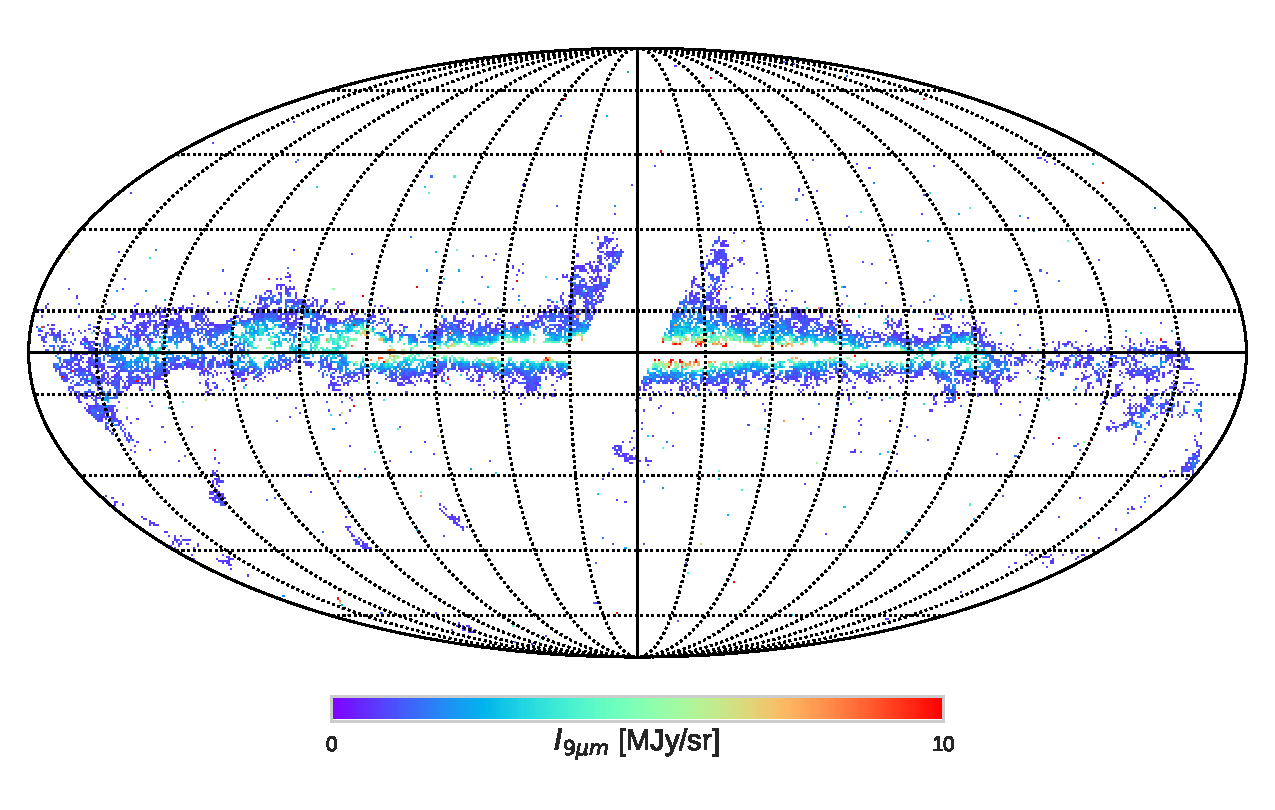
\includegraphics[width=\textwidth]{../Plots/ch_allsky/masked_map_A9.pdf}
          \centering
          \caption{All-sky map in A9 emission after applying the combined masks: ecliptic plane, galactic plane, point sources, and pixels with S/N $<1$. This mask essentially outlines the galaxy, except for the most confused regions.}
          \label{fig:A9_masked_map}
        \end{figure}
         Fig.~\ref{fig:AMEvsDust_allsky_allbands_mpsub_kde_masked} shows point-density plots for $AME_{var}$ vs. each of the IR bands, after applying the mask described above.
            \begin{figure}
              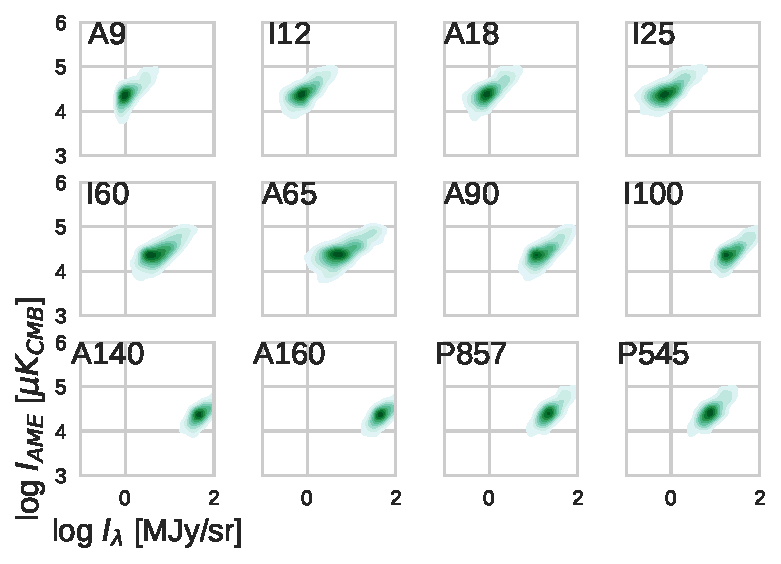
\includegraphics[width=\textwidth]{../Plots/ch_allsky/AMEvsDust_allsky_allbands_mpsub_kde_masked.pdf}
              \centering
              \caption{The same comparison as shown for Fig.~\ref{fig:AMEvsDust_allsky_allbands_mpsub_kde_unmasked}, but with the mask applied as in Fig.~\ref{fig:A9_masked_map}.}
              \label{fig:AMEvsDust_allsky_allbands_mpsub_kde_masked}
            \end{figure}
          As expected with such a drastic reduction of the number of noise-dominated points, the scatter, especially for the MIR bands, is reduced. Otherwise the applicaiton of the mask does not bring about any special distinction among the bands when compared to the AME. What is notable however is that the persistent weakening of trend of I25 vs. AME, relative to A9 and the FIR bands. Following the logic that the PAH-tracing bands intensity is essentially a product of the ISRF ($U$) and the column density of PAHs ($\sigma_{PAH}$), we redraw the comparison after scaling the IR bands by $U$. We do this not only for the MIR bands, simply for comparison. We do not have a theoretical prediction as to the relationship between AME intensity and the FIR bands' intensities scaled by $U$. The pixel density plots for such a comparison are given by Fig.~\ref{fig:AMEvsDust_allsky_allbands_mpsub_UNorm_kde_masked}, which is the same as Fig.~\ref{fig:AMEvsDust_allsky_allbands_mpsub_kde_masked} except for division of the X-axes by $U$.
            \begin{figure}
              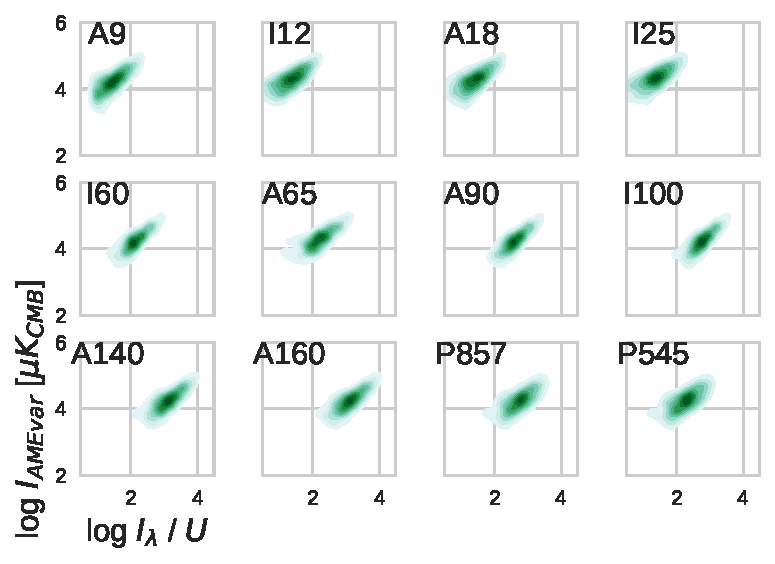
\includegraphics[width=\textwidth]{../Plots/ch_allsky/AMEvsDust_allsky_allbands_mpsub_UNorm_kde_masked.pdf}
              \centering
              \caption{Similar comparison to Fig.~\ref{fig:AMEvsDust_allsky_allbands_mpsub_kde_unmasked}, with the IR intensities scaled by $U$ for each pixel. }
              \label{fig:AMEvsDust_allsky_allbands_mpsub_UNorm_kde_masked}
            \end{figure}
          Corresponding to the plots vs. AME given in Figs. Fig.~\ref{fig:AMEvsDust_allsky_allbands_mpsub_UNorm_kde_masked} and~\ref{fig:AMEvsDust_allsky_allbands_mpsub_kde_masked}, we again perform a cross-correlation matrix test, to understand how the bands relate to one another- not only to the AME. This cross-correlation is done for both intensity, shown by Fig.~\ref{fig:all_bands_corr_matrix_wAME_spearmanintensity_maskall} and $U$ normalized intensities showin in Fig.~\ref{fig:all_bands_corr_matrix_wAME_spearmanU_norm_masked}.
            \begin{figure}
              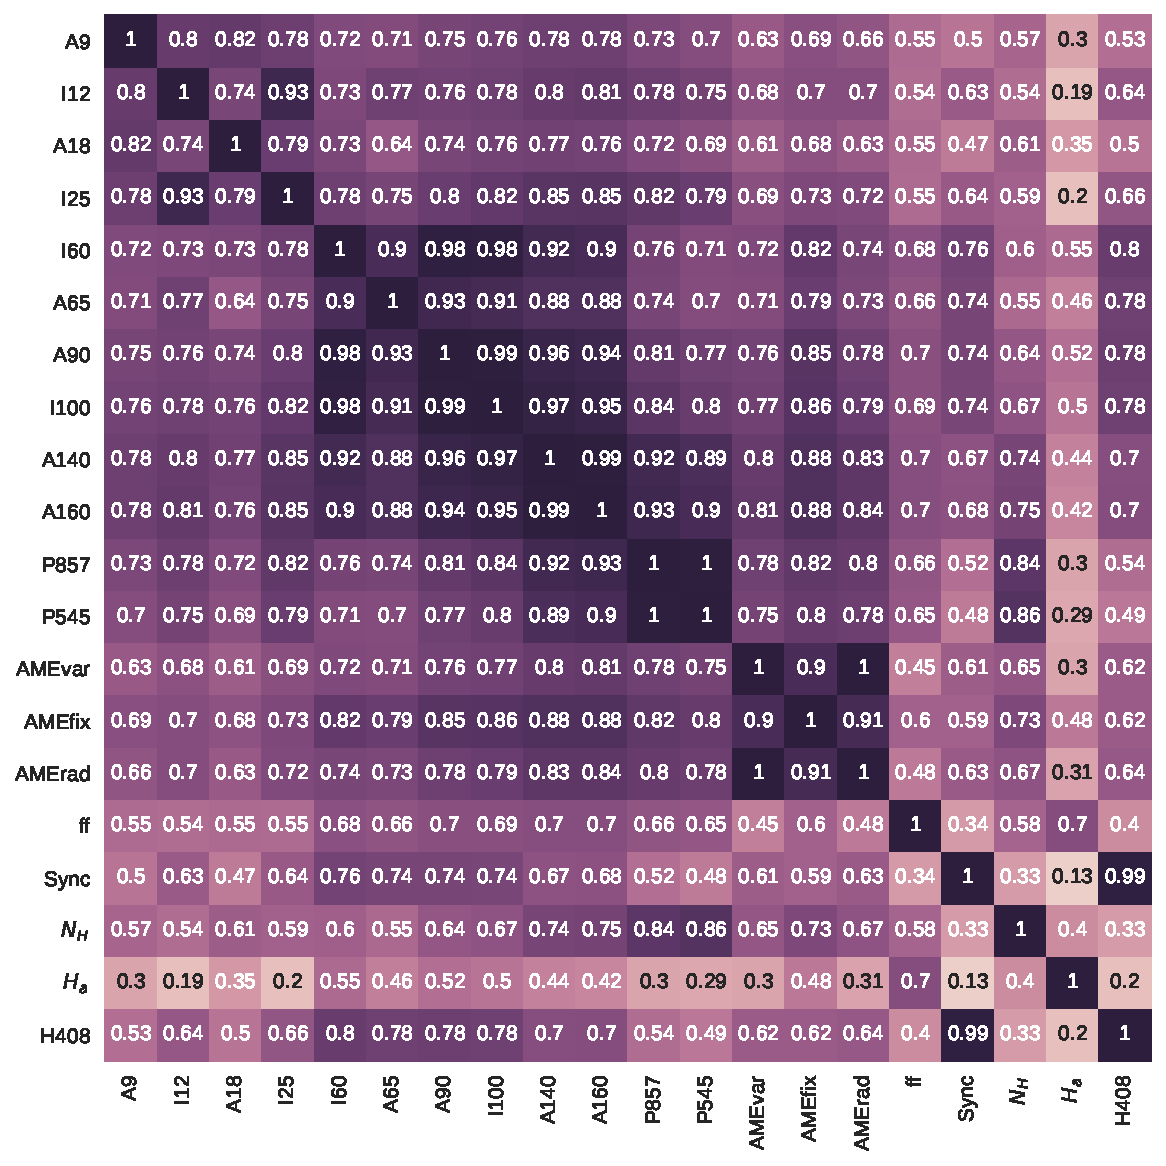
\includegraphics[width=\textwidth]{../Plots/ch_allsky/all_bands_corr_matrix_wAME_spearmanintensity_maskall.pdf}
              \centering
              \caption{Cross-correlation ($r_{s}$ matrix for the IR intensities (unscaled) vs. each other, esssentially the same comparison as in Fig.~\ref{fig:all_bands_corr_matrix_wAME_spearman}, except that the pixel mask is applied.}
              \label{fig:all_bands_corr_matrix_wAME_spearmanintensity_maskall}
            \end{figure}
            \begin{figure}
              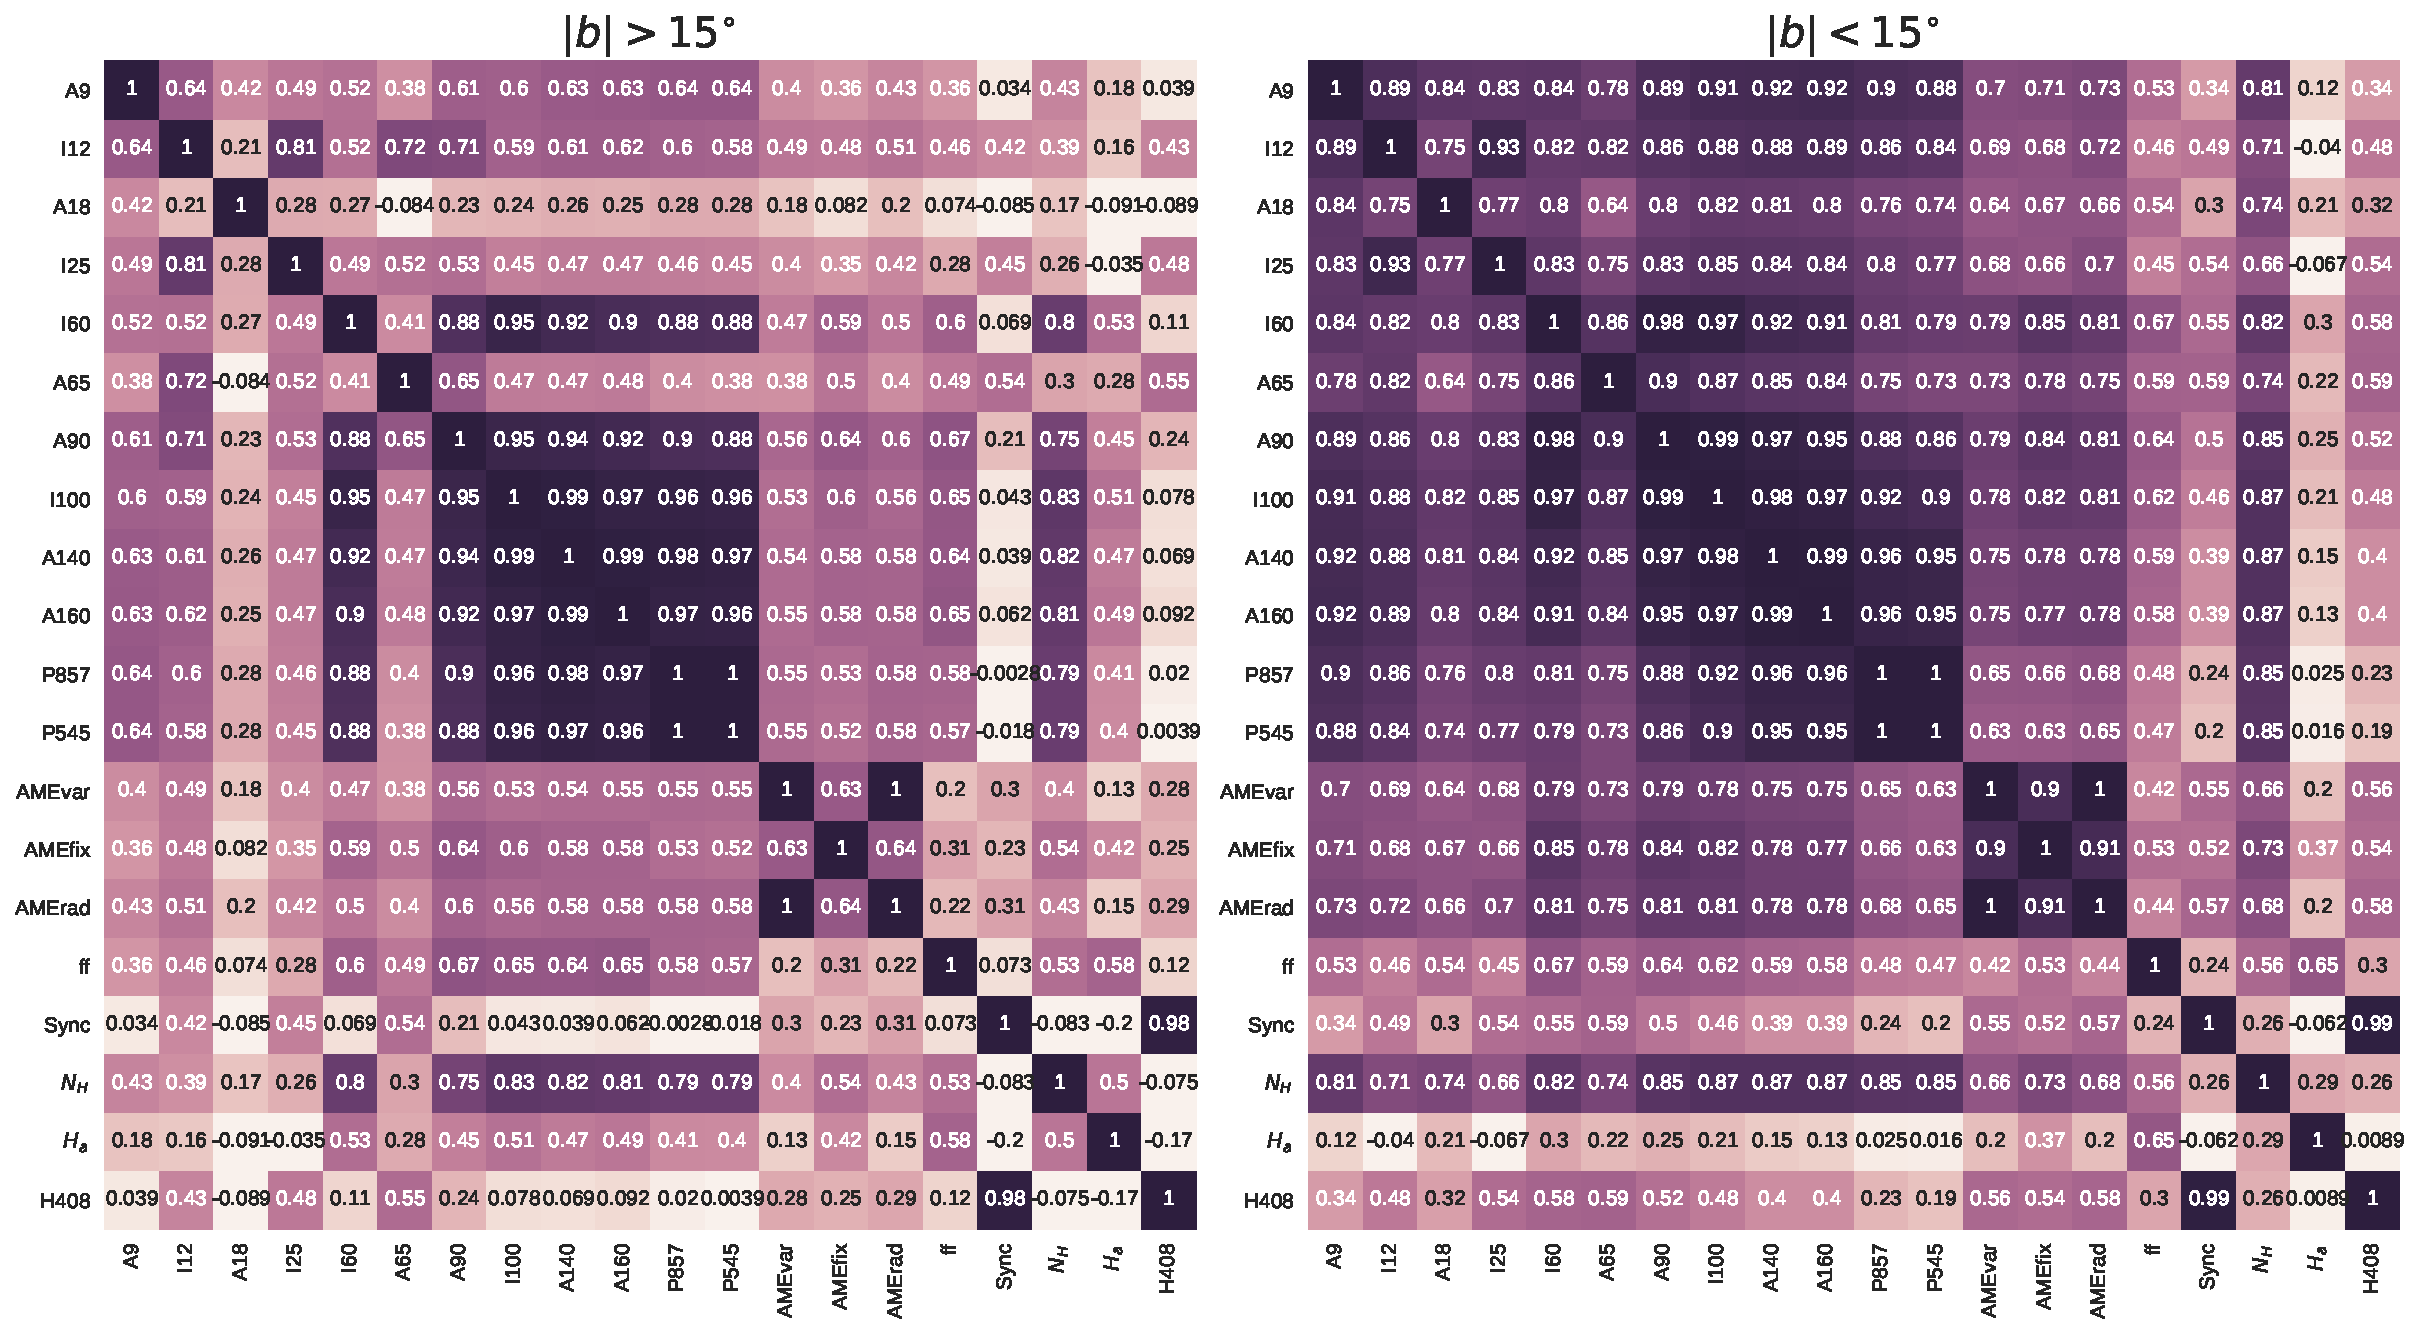
\includegraphics[width=\textwidth]{../Plots/ch_allsky/all_bands_corr_matrix_wAME_spearmanU_norm_masked.pdf}
              \centering
              \caption{Cross-correlation ($r_{s}$ matrix for the $U$-normalized IR intensities vs. each other, and also against the AME components, other PC products, and ancilliary data. Only the IR maps are divided by $U$- other data is unchanged from Fig.~\ref{fig:all_bands_corr_matrix_wAME_spearmanintensity_maskall})}
              \label{fig:all_bands_corr_matrix_wAME_spearmanU_norm_masked}
            \end{figure}

        \paragraph{Bootstrap test}
            In addition, for the masked comparison, we carry out a boostrap analysis similar to that discussed in Ch.~\ref{ch:lori} and Fig.~\ref{fig:bootstrap_vs_AME}. The Spearman rank correlation coefficents $r_{S}$ of all of the bands, in intensity, vs. the $AME{var}$ component are shown. This is done only for the masked case, due to the computational challeneges presented by a well-sampled bootstrap of all ~700,000 pixels in the full sky. Because the mask applied here leaves us with approximately 1/7 of the sky, a bootstrap of N iterations with N pixels becomes tractable (though ideally we would prefer $n_{iterations} > n_{samples}$). We show the comparison only for the $AME_{var}$ component also due to computational constraints. The $r_{s}$ distributions for each IR band vs. AME are shown in Fig.~\ref{fig:bootstrap_vs_AME_allsky_masked}
            \begin{figure}
                 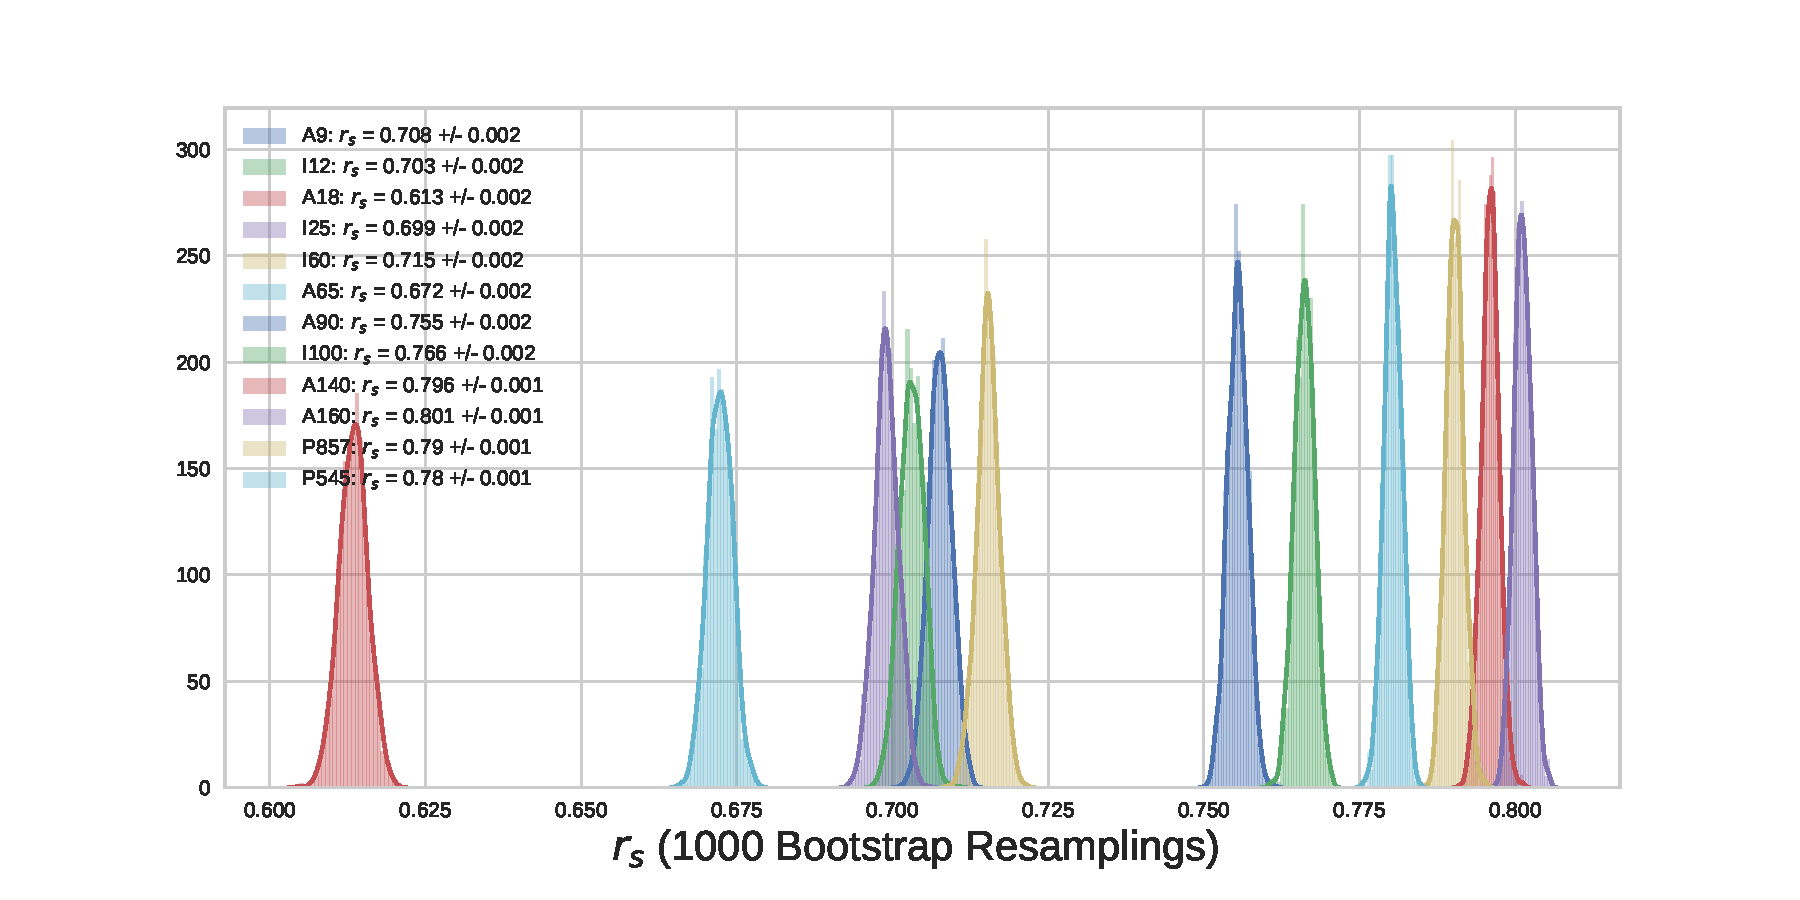
\includegraphics[width=\textwidth]{../Plots/ch_allsky/bootstrap_vs_AME_spearman_maskall_i1000.pdf}
                 \centering
                 \caption{.}
                 \label{fig:bootstrap_vs_AME_allsky_masked}
            \end{figure}

  \section{Spatial variaton of correlations}
    To understand how these trends may vary across the sky, we produce an all-sky maps of $r_{s}$ for AME vs. IR emission. From the NSIDE~256 input maps of AME and 4 IR wavelength maps, we produce NSIDE~8 maps of $r_{s}$. These maps are shown in Figs.~\ref{fig:Spearman_Map_nside8_AMEtoIR_A9} and~\ref{fig:Spearman_Map_nside8_AMEtoIR_I12}.
      \begin{figure}
        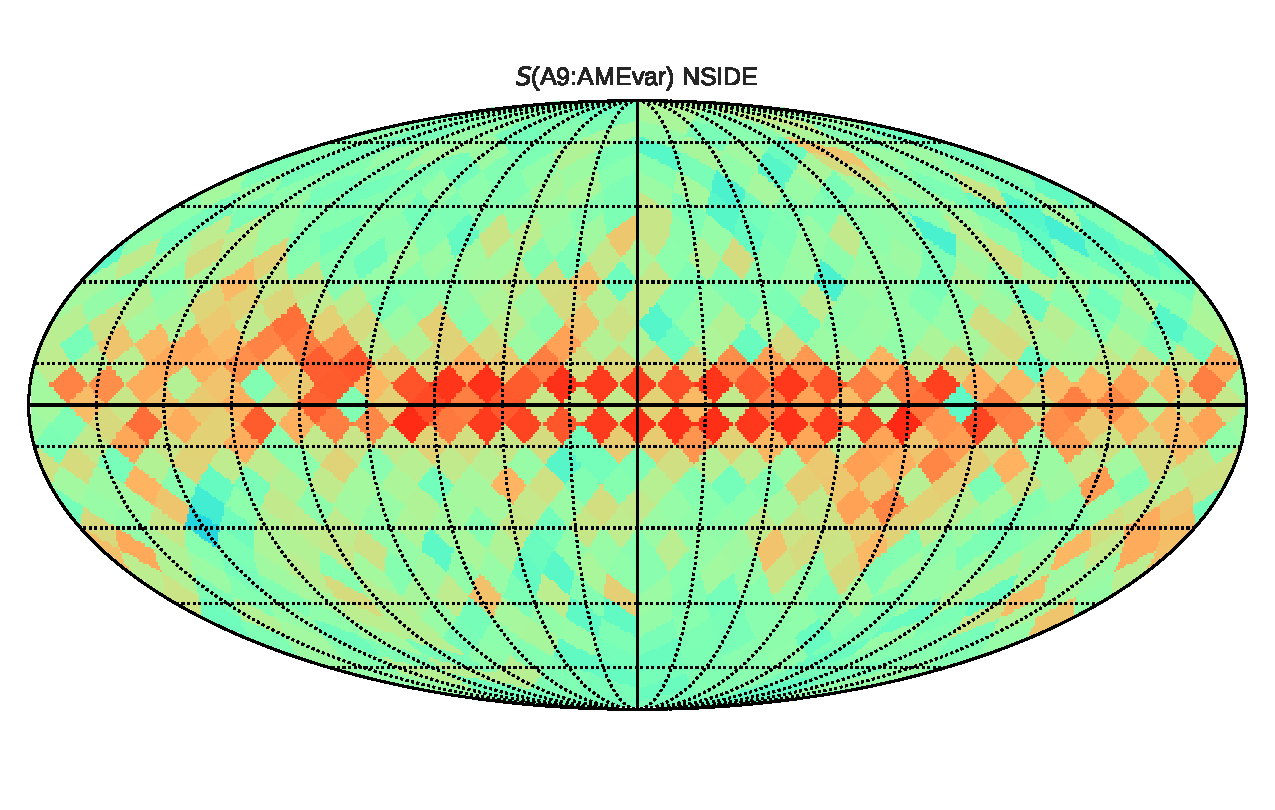
\includegraphics[width=\textwidth]{../Plots/Allsky_Corr/Spearman_Map_nside8_A9toAMEvar.pdf}
        \centering
        \caption{Spatial map of $r_{s}$ between the AME and IR intensity for 4 bands:$9~\mu{}m$, $12~\mu{}m$, $25~\mu{}m$, and $140~\mu{}m$. $r_{s}$ is calculated for all NSIDE~256 pixels within each NSIDE~8 pixel-sized bin.}
        \label{fig:Spearman_Map_nside8_AMEtoIR_A9}
      \end{figure}
      \begin{figure}
        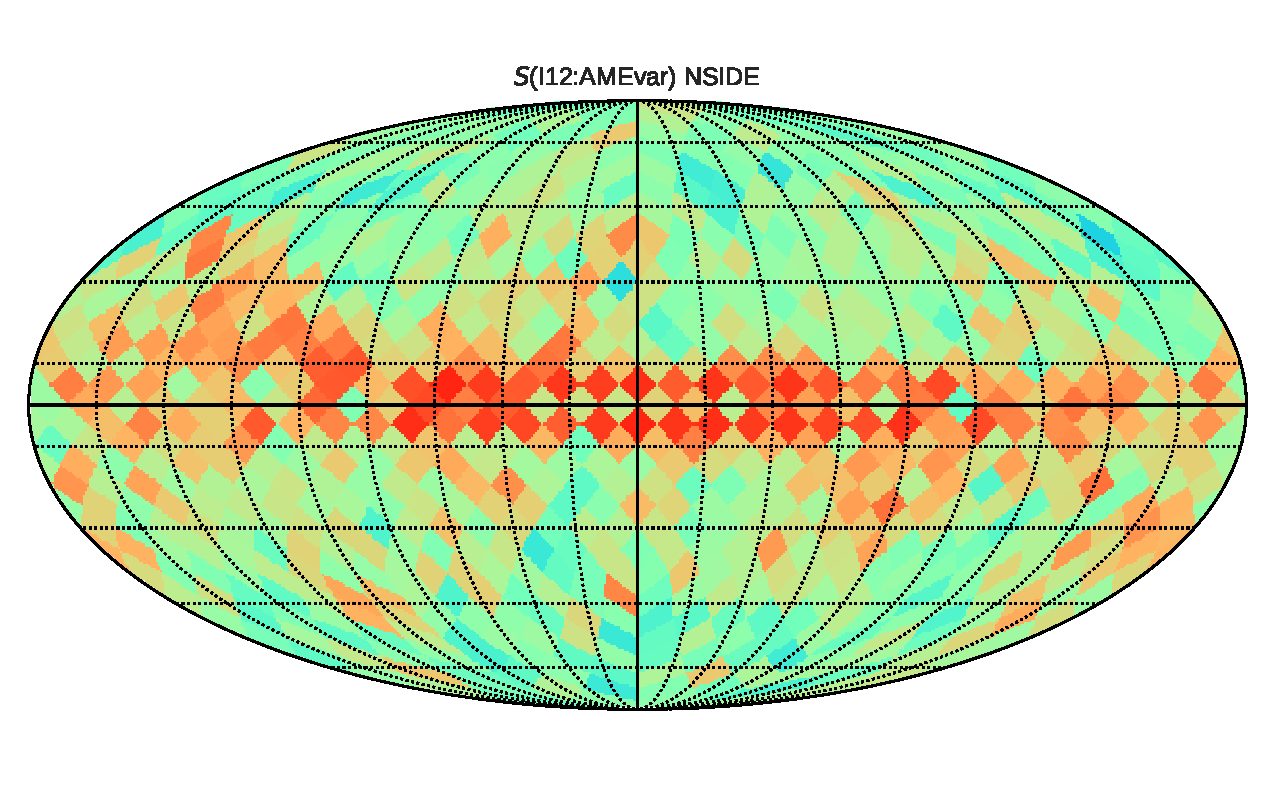
\includegraphics[width=\textwidth]{../Plots/Allsky_Corr/Spearman_Map_nside8_I12toAMEvar.pdf}
        \centering
        \caption{}
        \label{fig:Spearman_Map_nside8_AMEtoIR_I12}
      \end{figure}
      \begin{figure}
        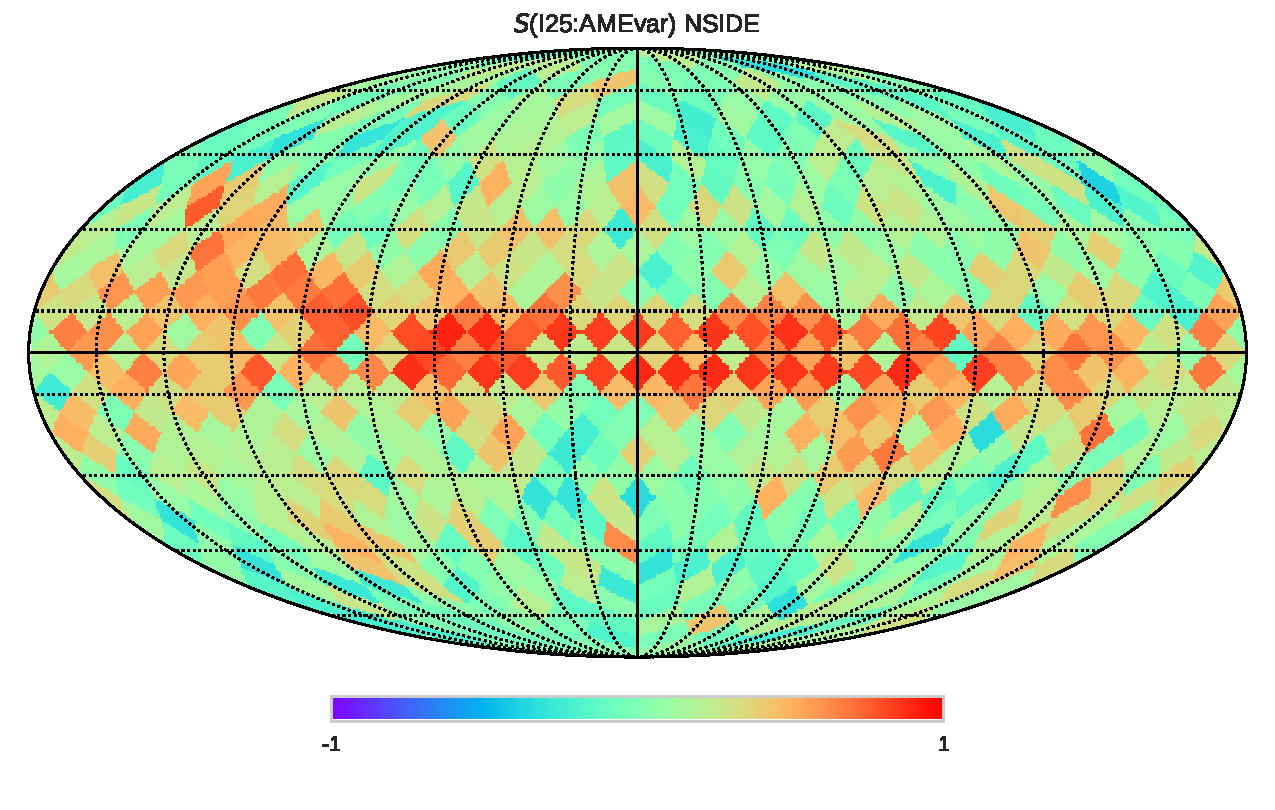
\includegraphics[width=\textwidth]{../Plots/Allsky_Corr/Spearman_Map_nside8_I25toAMEvar.pdf}
        \centering
        \caption{}
        \label{fig:Spearman_Map_nside8_AMEtoIR_I25}
      \end{figure}
      \begin{figure}
        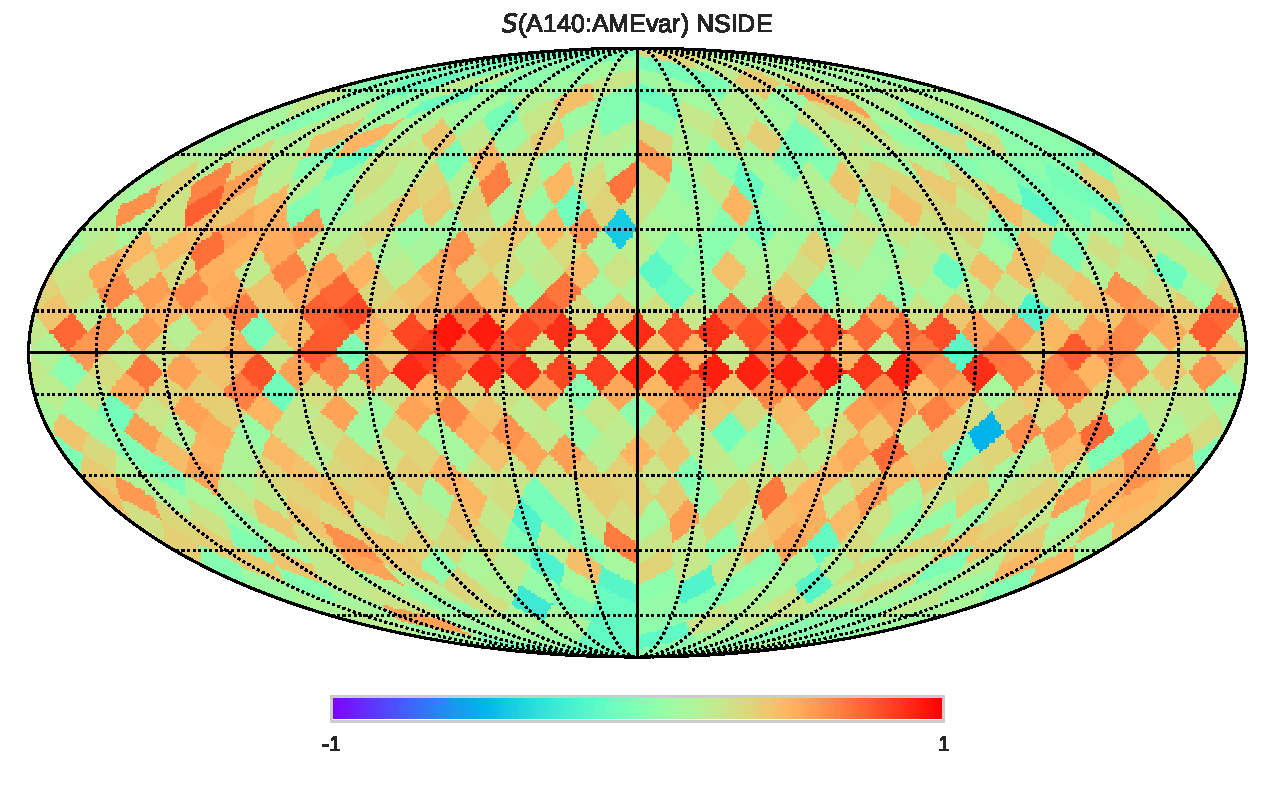
\includegraphics[width=\textwidth]{../Plots/Allsky_Corr/Spearman_Map_nside8_A140toAMEvar.pdf}
        \centering
        \caption{}
        \label{fig:Spearman_Map_nside8_AMEtoIR_A140}
      \end{figure}

     \begin{figure}
       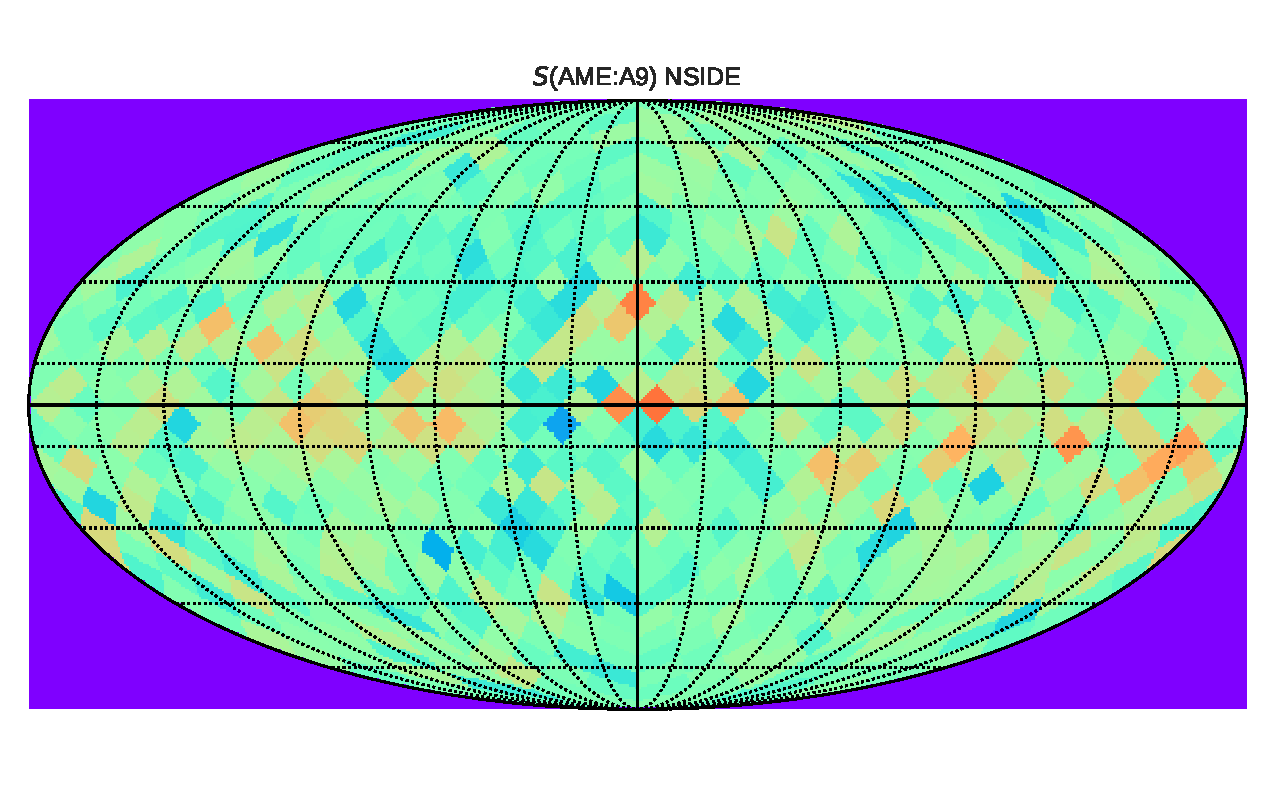
\includegraphics[width=\textwidth]{../Plots/Allsky_Corr/RadNorm/Spearman_Map_nside8_AMEtoA9.pdf}
       \centering
       \caption{Spatial map of $r_{s}$ between the AME and IR intensity as in Fig.~\ref{fig:Spearman_Map_nside8_AMEtoIR}, but with the AME and IR maps first normalized y dust radiance $R$.}
       \label{fig:Spearman_Map_nside8_AMEtoIR_radnorm_A9}
      \end{figure}
       \begin{figure}
        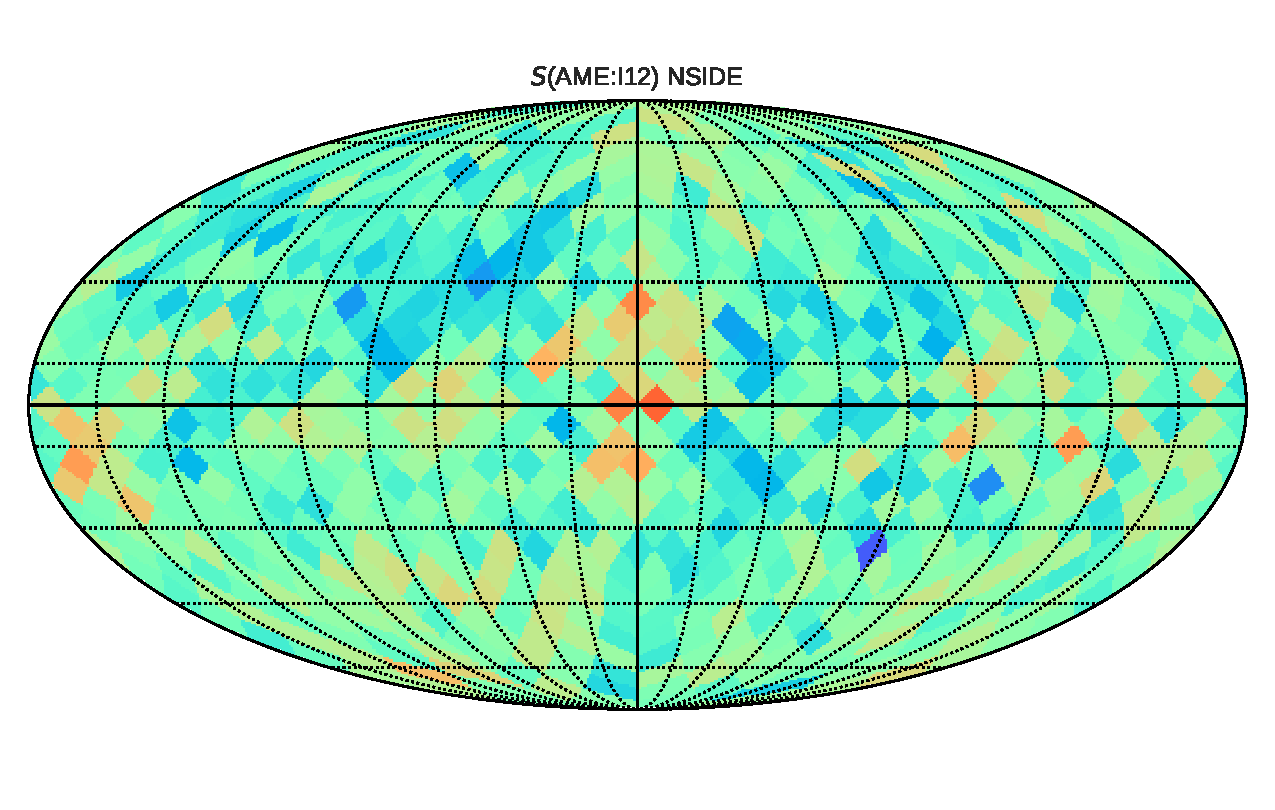
\includegraphics[width=\textwidth]{../Plots/Allsky_Corr/RadNorm/Spearman_Map_nside8_AMEtoI12.pdf}
        \centering
        \caption{}
        \label{fig:Spearman_Map_nside8_AMEtoIR_radnorm_I12}
      \end{figure}
        \begin{figure}
         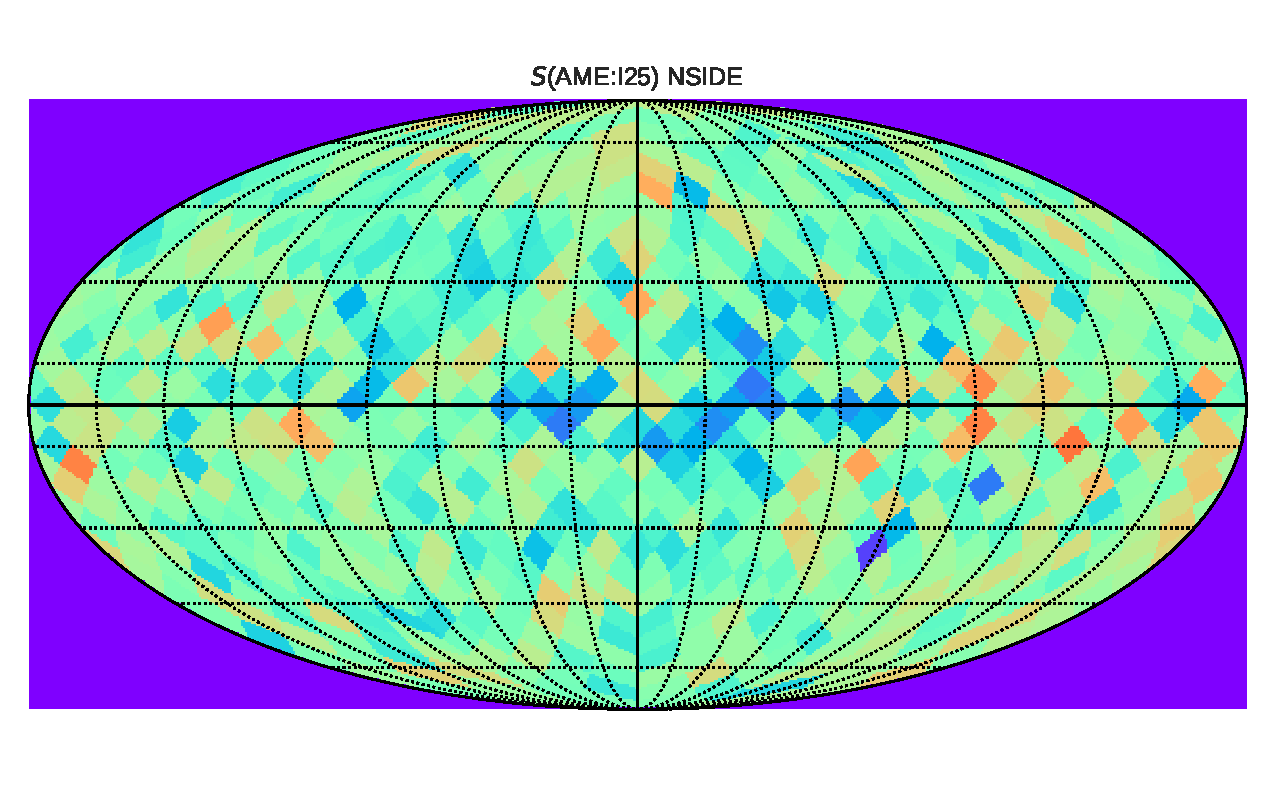
\includegraphics[width=\textwidth]{../Plots/Allsky_Corr/RadNorm/Spearman_Map_nside8_AMEtoI25.pdf}
         \centering
         \caption{}
         \label{fig:Spearman_Map_nside8_AMEtoIR_radnorm_I25}
      \end{figure}
        \begin{figure}
        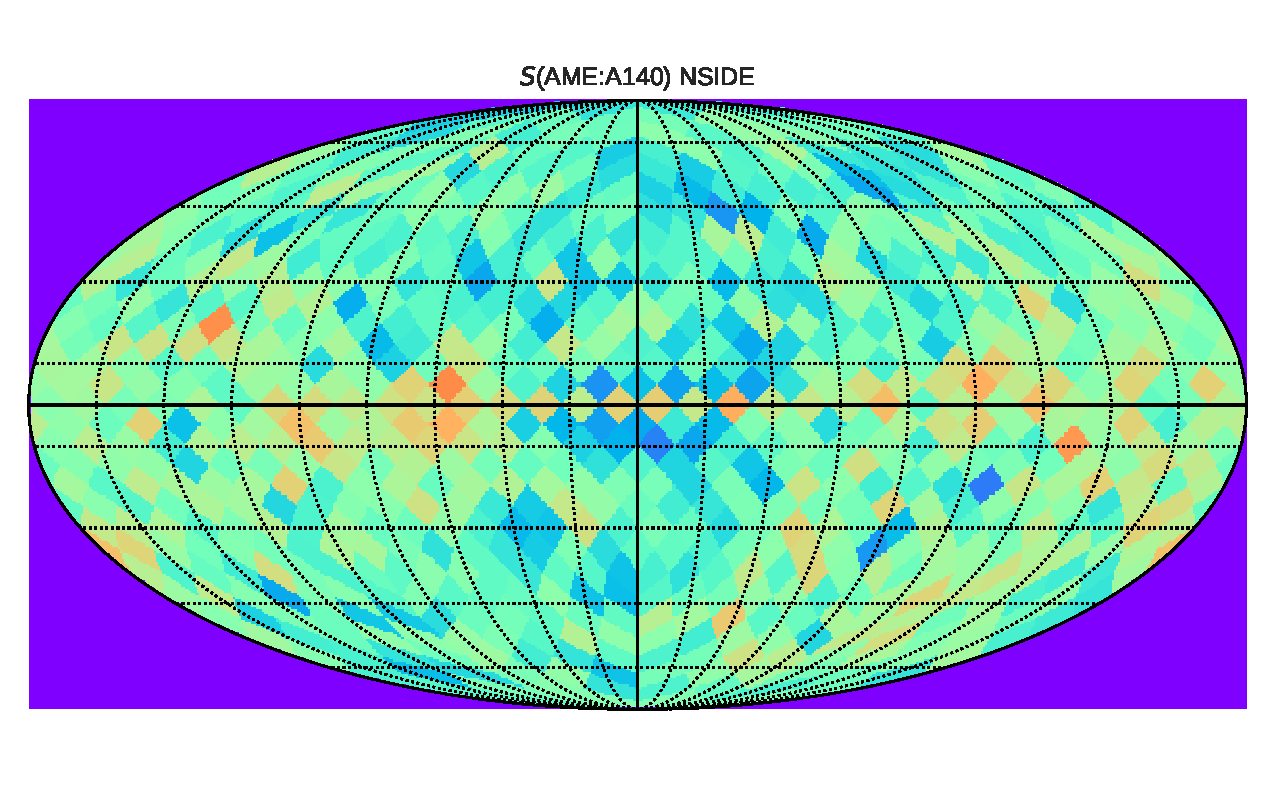
\includegraphics[width=\textwidth]{../Plots/Allsky_Corr/RadNorm/Spearman_Map_nside8_AMEtoA140.pdf}
        \centering
        \caption{}
        \label{fig:Spearman_Map_nside8_AMEtoIR_radnorm_A140}
        \end{figure}


    \section{Discussion}
      \subsection{AME:Dust}
        As noted in Ch. \hyperref[ch:intro]{\ref{ch:intro}}, previous studies found that the AME generally correlates at dust-related IR wavelengths \citep{ysard10b,planckXV, hensley16}. We see the same overall pattern in the present study.

         In our all-sky comparison, we find a first-order correlation between IR intensity and AME intensity, for each of the 12 wavelengths sampled. This is again consistent with the previous investigations of the AME cited above, in that the FIR emission shows the tightest correlation with the AME intensity.

         In testing for a second-order correlation, we divided the IR intensities and AME intensity by the dust radiance, and again performed the band-by-band all-sky comparison. There is evidence of a residual correlation between $I_{MIR}$ and $I_{AME}/R$. Unsurprisingly, the strong correlation between $I_{FIR}$ and $I_{AME}$ disappears when scaling by $R$, as the the FIR bands are dominated by thermal dust emission. In this case, we again find no evidence of an improved correlation for the PAH-dominated bands.

           The closeness of the correlation coefficients found here is consistent with the results of the IRAS vs. AME correlation test result from \cite{planckXV}. They found that the correlation coefficient among the 4 IRAS bands (12, 25, 60, and 100~$\mu$m) differ from one another only by about 5\%, across the whole set of 98 regions. The trend of AKARI MIR and FIR data vs. the AME does not disagree with their IRAS comparison. This work adds that bands longer than IRAS 100~$\mu$m also correlate strongly with AME, especially the two Planck/HFI bands used.

          \subsection{AME:PAH}
            Each of the bands sampled show correlation with the AME, however the FIR bands always show the strongest correlation. In fact, the correlation pattern of AME vs. each of the IR bands, very strongly resembles the correlation results of the FIR vs. all of the other maps. This is readily apparent from the pixel-density plots in Figs.~\ref{fig:AMEvsDust_allsky_allbands_mpsub_kde_unmasked} and~\ref{fig:AMEvsDust_allsky_allbands_mpsub_kde_masked}, wherein the FIR bands pixels show a very similar density profile vs. the AME. In attempting to factor out this first-order correlation, dividing the AME and IR intensities by $U$ for each pixel, we find the there is still a residual correlation between the MIR bands and the AME.

          \subsection{AME:$T$, $G_{0}$}
            According to spinning dust theory outlined in \cite{draine98a} and in subsequent works by \cite{ysard10a}, the AME profile and intensity will depend in part on the ISRF- but as is well-stated in \cite{hensley17a}, exactly how the ISRF will affect the AME SED is a more complicated question. Absorbed starlight photons may be able to rotationally excite the carriers, but if an enhanced ISRF leads to increased dust heating, then the increased IR emission can rotationally de-excite the carriers. Moreover the ISRF affects not only the dust temperature but ionization of the carriers.

            %\cite{hensley16} looked at the $AME$/$R$ ratio vs. $T$ and found only a slight anti-correlation of $P = -0.06$.

          \subsection{Microwave foreground component separation}

            There are known degeneracies between the foreground parameters of the COMMANDER maps (spinning-dust, and free-free, synchrotron components as described in \cite{planck15X}.) This can be demonstrated by comparing the ratio map of the PCXV intensity to thermal dust intensity.
